% Copyright (C) 2019 Cui Jialiang ( SESS, PKU ). All rights reserved.

\chapter{深度学习理论与现有的视频目标跟踪算法概论}
本章将介绍深度学习与视频目标跟踪算法的基础概念与常用算法.
\par
深度学习是本研究运用的主要方法,但其并不是本人专业常用的方法.本研究为了利用计算机学最新的研究成果,研究并采用了计算机视觉,统计领域今年来常用的深度学习方法.本研究提出的算法也将主要由多种深度学习算法组合而成.
\par
本章还将介绍一些视频目标跟踪算法.
\section{深度学习基础概念}
深度学习(Deep Lrarning)是以深度神经网络为模型结构的机器学习算法\supercite{deng2014deep}.机器学习(Mechine Learning)通常指一些依靠计算机确定模型的建模方法.目前大多数机器学习算法还无法完全自行实现学习,通常只能在人为规定的模型下,针对某个小问题对特定的数据建模.
\par
机器学习,模式识别等学科最终试图解决的问题通常是建立模型,解决问题.如目标跟踪即可描述为输入是视频,输出是轨迹的问题.神经网络(Neural Network, NN)由于其优秀的非线性拟合能力,成为如今机器学习最常用的模型结构之一.
\subsection{神经网络}
神经网络最初的灵感一部分来源于仿生学\supercite{mcculloch1943logical}\supercite{farley1954simulation},这也是神经网络的灵魂思想.
\par
相比于k-NN,SVM(支持向量机),线性回归(linear regression)等传统机器学习算法,神经网络主要依靠激活函数(activation function)得到非线性效果.为了避免梯度消失的问题,近期的研究与应用中最常用的激活函数是ReLU激活函数\supercite{krizhevsky2012imagenet}.不同的激活函数会有不同效果\supercite{karlik2011performance}.
\par
而相比与各种树模型,神经网络又有更好的泛华能力.
\par
\subsubsection{全链接神经网络}
\par
最简单的神经网络结构是全连接的(Fully Connected, 简称FC)神经网络, 该结构又称多层感知机(Multi Layer Perceptron, 简称MLP).多层感知机由多个层$l_1,l_2,...l_n$依次排列组成.每个层由许多神经元组成,某以层上的每个神经元将接受上一层所有神经元为输入,并向下一层的所有神经元输出.以ReLU为激活函数,位第k层的第m个神经元的输出为$output_{k,m}=ReLU(\sum_{i} (output_{k-1,i}*w_{k,m,i})+b_{k,m})$,其中$w_{k}$和$b_{k}$是属于第k层的变量,通常经过训练得出.
\par
全连接神经网络的连接较多,参数也会更多,即所有参数组成的参数向量很稀疏,不利于训练.通常只在最终将多维的状态量收敛成低维结果时使用.在前期对高维的数据的处理过程中,常常会对神经网络的结构进行一定简化,减少连接以利于训练.常用的减少连接方式有卷积神经网络和循环神经网络等.
\par
\subsubsection{卷积神经网络}
\par
\begin{figure}[htbp!]
    \centering
    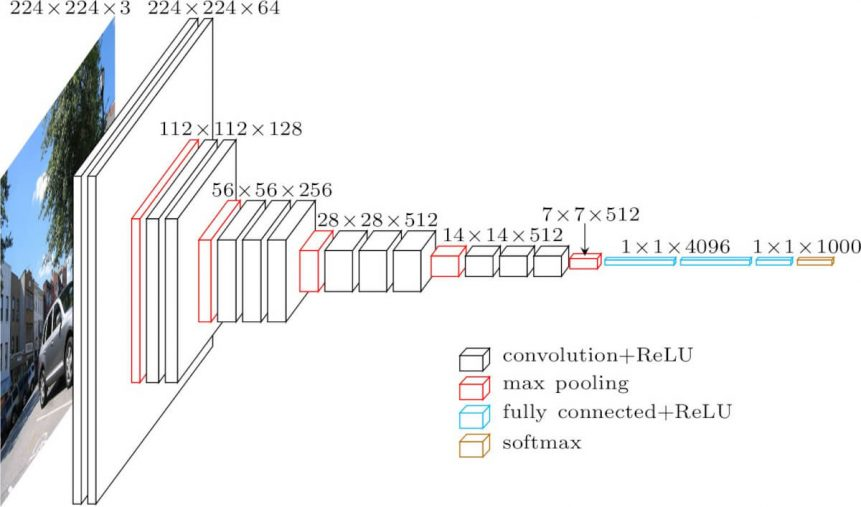
\includegraphics[width = 1.\textwidth]{chap/img/vgg16-neural-network.jpg}
    \caption{
        用于图像分类的VGG16\supercite{simonyan2014very}卷积神经网络结构图.图片来自 \url{https://neurohive.io/en/popular-networks/vgg16/}
        }\label{fig:vgg16_architecture}
\end{figure}
\par
卷积神经网络(Convolutional Neural Network, 简称CNN)是一种为图像处理设计的神经网络结构.同全连接神经网络一样,卷积神经网络也分为很多层,每一层只与前一层和后一层连接.不同的是,每层的一个神经元只连接前一层与后一层的少部分神经元.通常,CNN的每一层可以用一个多波段图像表示,连接只建立在前一层与后一层位置接近的像素上.类似图像处理中的模板滤波方法.常用的CNN的模板大小是$3*3$,有时也可以是$5*5$,$7*7$等大小.每一层的所有神经元公用一个模版,模版上所有的参数都是训练得到的变量.卷积神经网络同样要在每层上加入激活函数,常用ReLU激活函数.
\par
完整的卷积神经网络通常会在卷积层中穿插池化(Pooling)层以收敛数据维度.池化层可以将卷积层图片大小减小.常用的配合ReLU激活函数的池化层如最大值池化(Max Polling)方法.以$2*2$为池的大小的池化层的输出为输入层大小的一半,每个像元为对应位置的4个像元的最大值.
\par
以图像分类问题为例,该问题需要输出一个较低维度的结果,即图像属于是每个类别的概率,可以用一个向量表示.用于图像分类的神经网络通常使用CNN层与最大值池化层交替减小图像大小,最终用全连接层得到分类结果.如图\ref{fig:vgg16_architecture}所示的VGG16\supercite{simonyan2014very}卷积神经网络即是这样一个图像分类算法.
\par
\begin{figure}[htbp!]
    \centering
    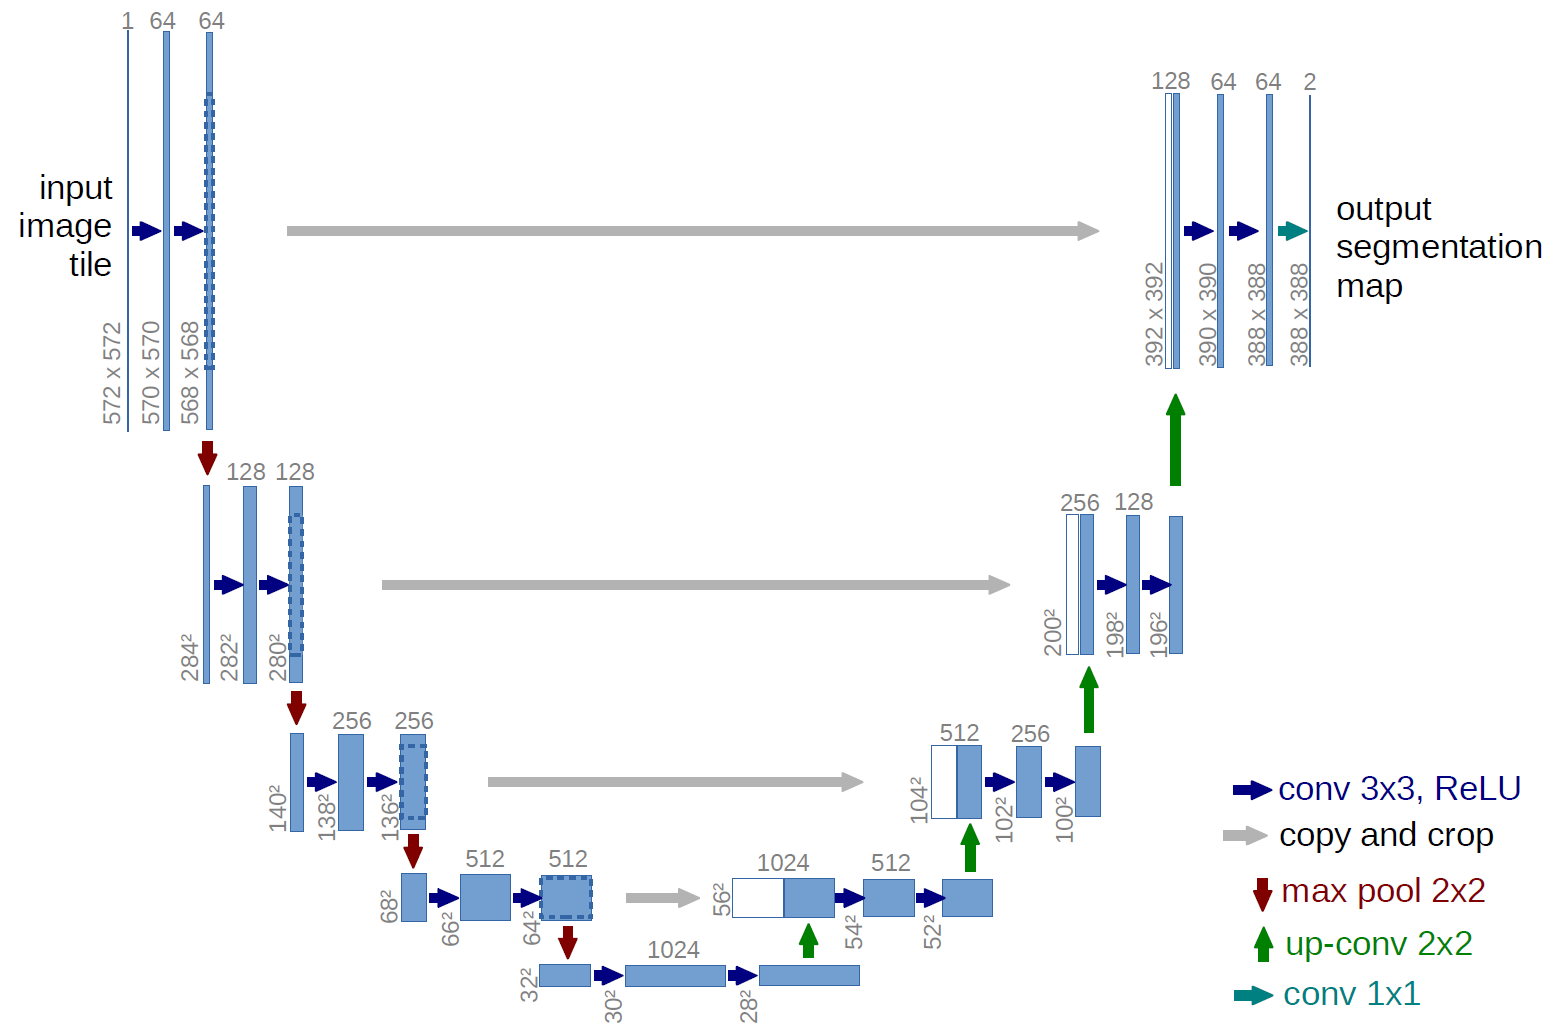
\includegraphics[width = 1.\textwidth]{chap/img/u-net-architecture.png}
    \caption{
        用于图像分割的U-Net\supercite{ronneberger2015u}卷积神经网络结构图.
        }\label{fig:unet_architecture}
\end{figure}
\par
不同于图像分类,图像分割等像素级图像处理问题需要得到更高维的结果,且得到的结果需要有一定的空间特性.如图\ref{fig:unet_architecture}的U-Net是一种常用的处理分割等像素级别问题的卷积神经网络.该网络有加密和解码两个步骤,加密阶段图像经过多次卷积和池化变小,蕴含的信息更宏观;而解码阶段图像经过反卷积(Deconvolution)操作再次放大,得到与原图大小相似的结果.类似的还有SegNet\supercite{badrinarayanan2017segnet}卷积神经网络等.
\par
U-Net的网络结构为像素级别处理提供了思想基础.
\par

\subsubsection{循环神经网络} \label{section:rnn}
RNN(循环神经网络, 又称递归神经网络, Recurrent Neural Network)是深度学习处理序列问题,尤其是时间序列数据时的重要方法.上文中介绍了全连接和卷积神经网络,这两种结构的神经网络接受的输入都是由网络结构事先确定的.如针对图像处理问题,通常的做法是将图片采样,拉伸至CNN的输入要求再进行处理.当进行时间序列分析时,这样的结构只能接受定长的时间序列数据.但实际上大多数时间序列数据是变长的.
\par
\begin{figure}[htbp!]
    \centering
    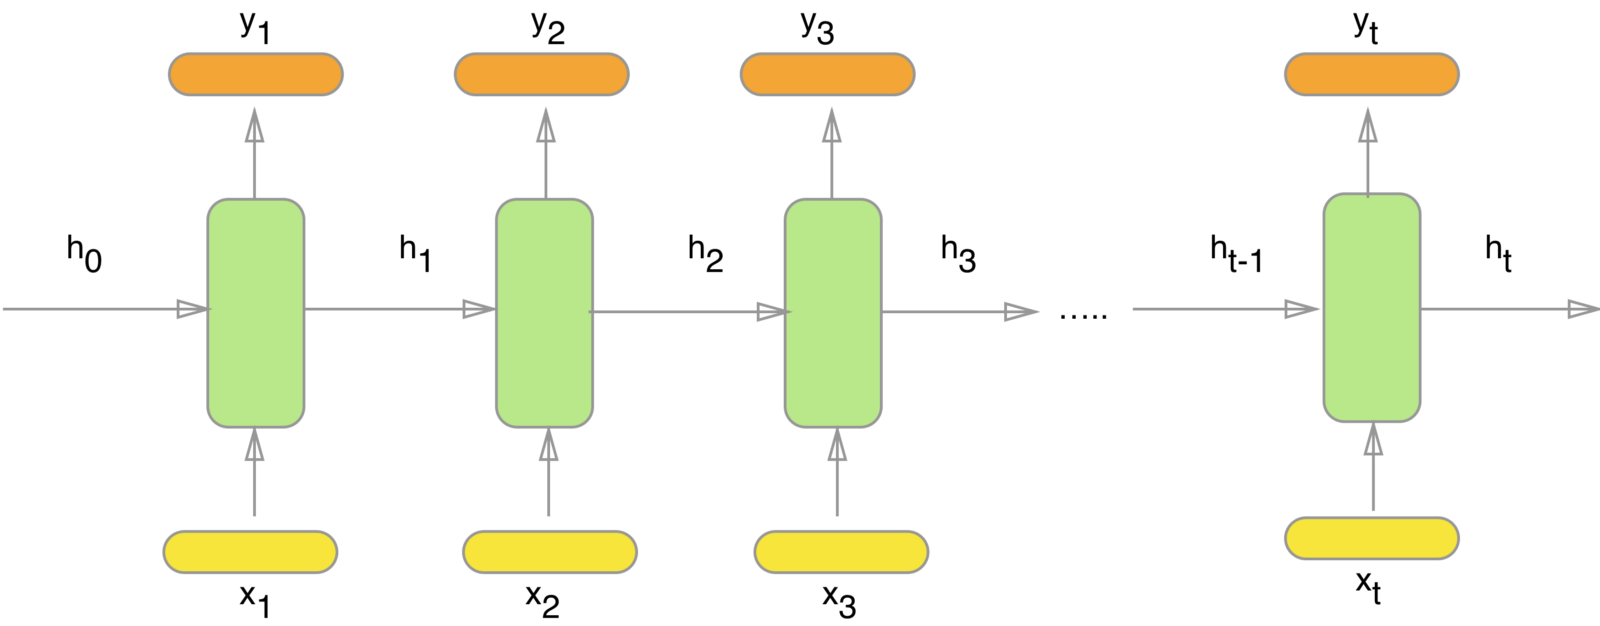
\includegraphics[width = 1.\textwidth]{chap/img/rnn.png}
    \caption{
        RNN的输入$x$,输出$y$与状态$h$的结构\supercite{how_rnn_work}
        }\label{fig:rnn}
\end{figure}
\par
RNN能很好解决这个问题.RNN可以将参数相同的某个神经单元重复使用多次以处理.通常情况下\footnote{这里介绍的RNN全是单向RNN,且对时间序列处理的先后顺序为时间流逝的顺序},RNN单元接受前一时刻的状态量和本时刻的信息,得到本时刻的输出和输出给下一时刻的状态量.
\par
如图\ref{fig:rnn}所示,对一个长度为$t$的时间序列,我们在每个时刻观察到的信息为$x_1, x_2, ...x_t$,则对第$i$时刻,有$y_i,h_i = RNN(x_i, h_{i-1})$.其中$y_i$为该时刻处理得到的结果,$h_i$为该时刻的状态描述即状态量,$RNN$为该RNN的处理函数,该RNN对每个时刻的处理函数参数相同.通常情况下,$x,y,h$都是张量.
\par
RNN可以得到和原序列一样变长结果,也可以得到定长的结果.通常变长的结果由每时刻的输出即上段的$y$组合得到,而定长的结果由最终的状态$h_t$经过处理得到.定长的结果一般用于该序列进行一个系统的描述,而变长的结果需要得到该序列每个时刻的信息.
\par
%TODO 介绍LSTM
%TODO 介绍RNN展开方式

\subsubsection{用于分类问题的神经网络结构}
\par
无论是FC,CNN还是RNN结果,神经网络在处理过程中传递的都是张量(Tensor\footnote{著名的深度学习框架Tensorflow\supercite{abadi2016tensorflow}即得名于此}).常见的矩阵(Matrix),向量(Vector)都是张量.如FC神经网络处理某条数据时,神经元数位$k$的某一层传给下一层的信息可以用大小为$k*1$的张量表示.这是这个量是一个向量.
\par
\begin{figure}[htbp!]
    \centering
    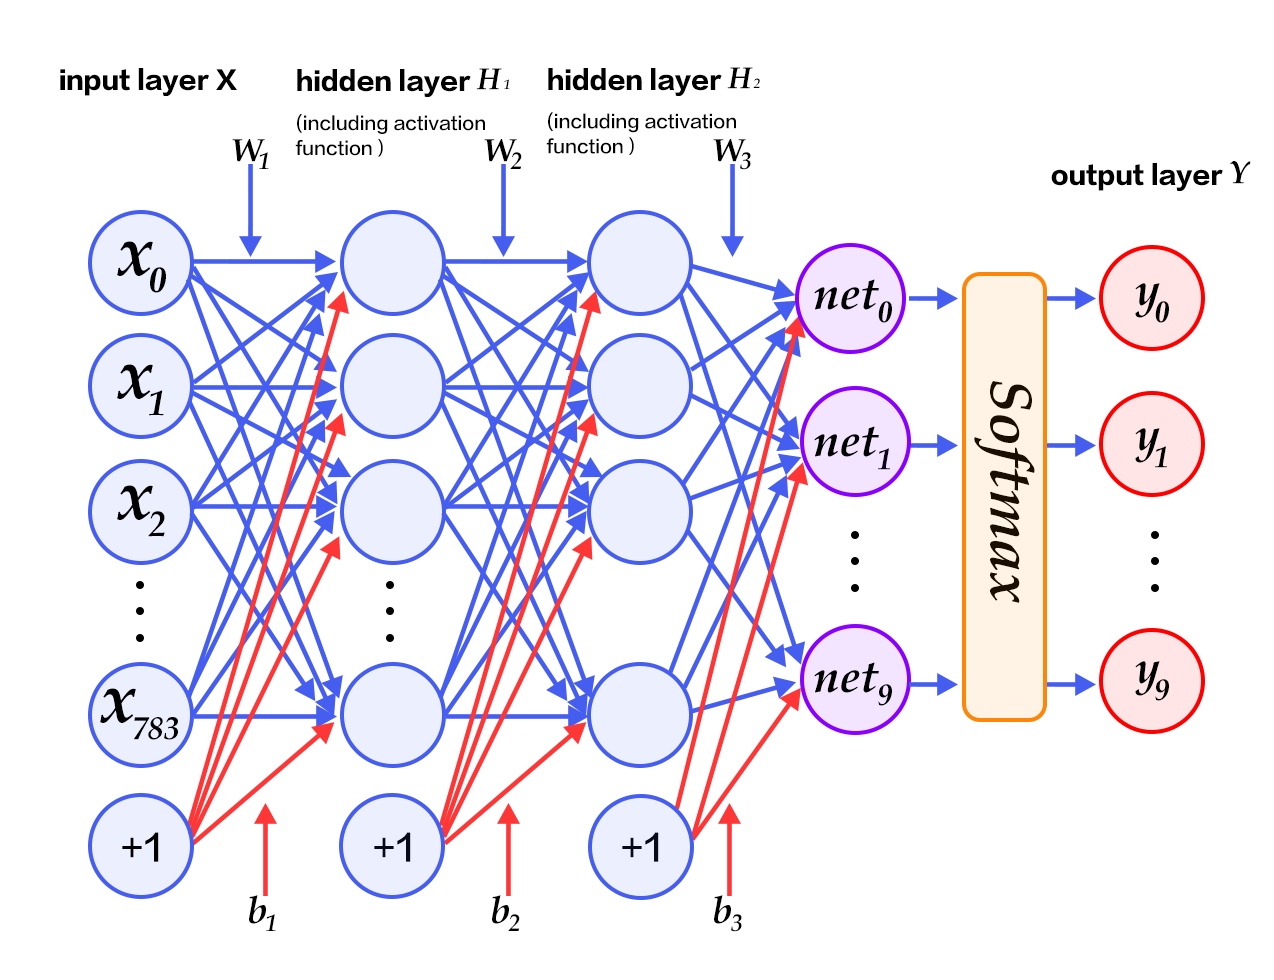
\includegraphics[width = 1.\textwidth]{chap/img/mlp_paddle.png}
    \caption{
        使用Softmax实现分类的多层神经网络,图片来自百度公司PaddlePaddle平台(\url{https://github.com/PaddlePaddle/Paddle})的文档\supercite{recognize_digits_paddle}
        }\label{fig:mlp_paddle}
\end{figure}
\par
图\ref{fig:mlp_paddle}即是一个用于分类问题的3层全连接神经网络,该分类问题需要将结果分为9类.第3层全链接层得到的结果可以记为$[net_0,net_1,...,net_9]$.解决分类问题时通常使用Softmax结构:
\par
\begin{equation} y_i = \frac{exp(net_i)}{\sum{ exp(net_i) }}  \end{equation}
\par
Softmax结构通常适用于多分类问题,而对于2分类问题,其简化版为Sigmoid函数:
\par
\begin{equation} y = \frac{1}{1+e^{-x}}  \end{equation}
\par
其中y是样本属于正例的概率, $y\in (0,1)$.
\par
需要注意的是,Softmax要求最后一个全连接层的输出宽度等于类别数量,而Sigmoid要求最后一个全链接层输出标量.且在使用Softmax和Sigmoid时,最后一个全连接层通常不含激活函数,如图\ref{fig:mlp_paddle}所示.

\subsubsection{深度神经网络的训练}
\par
\begin{figure}[htbp!]
    \centering
    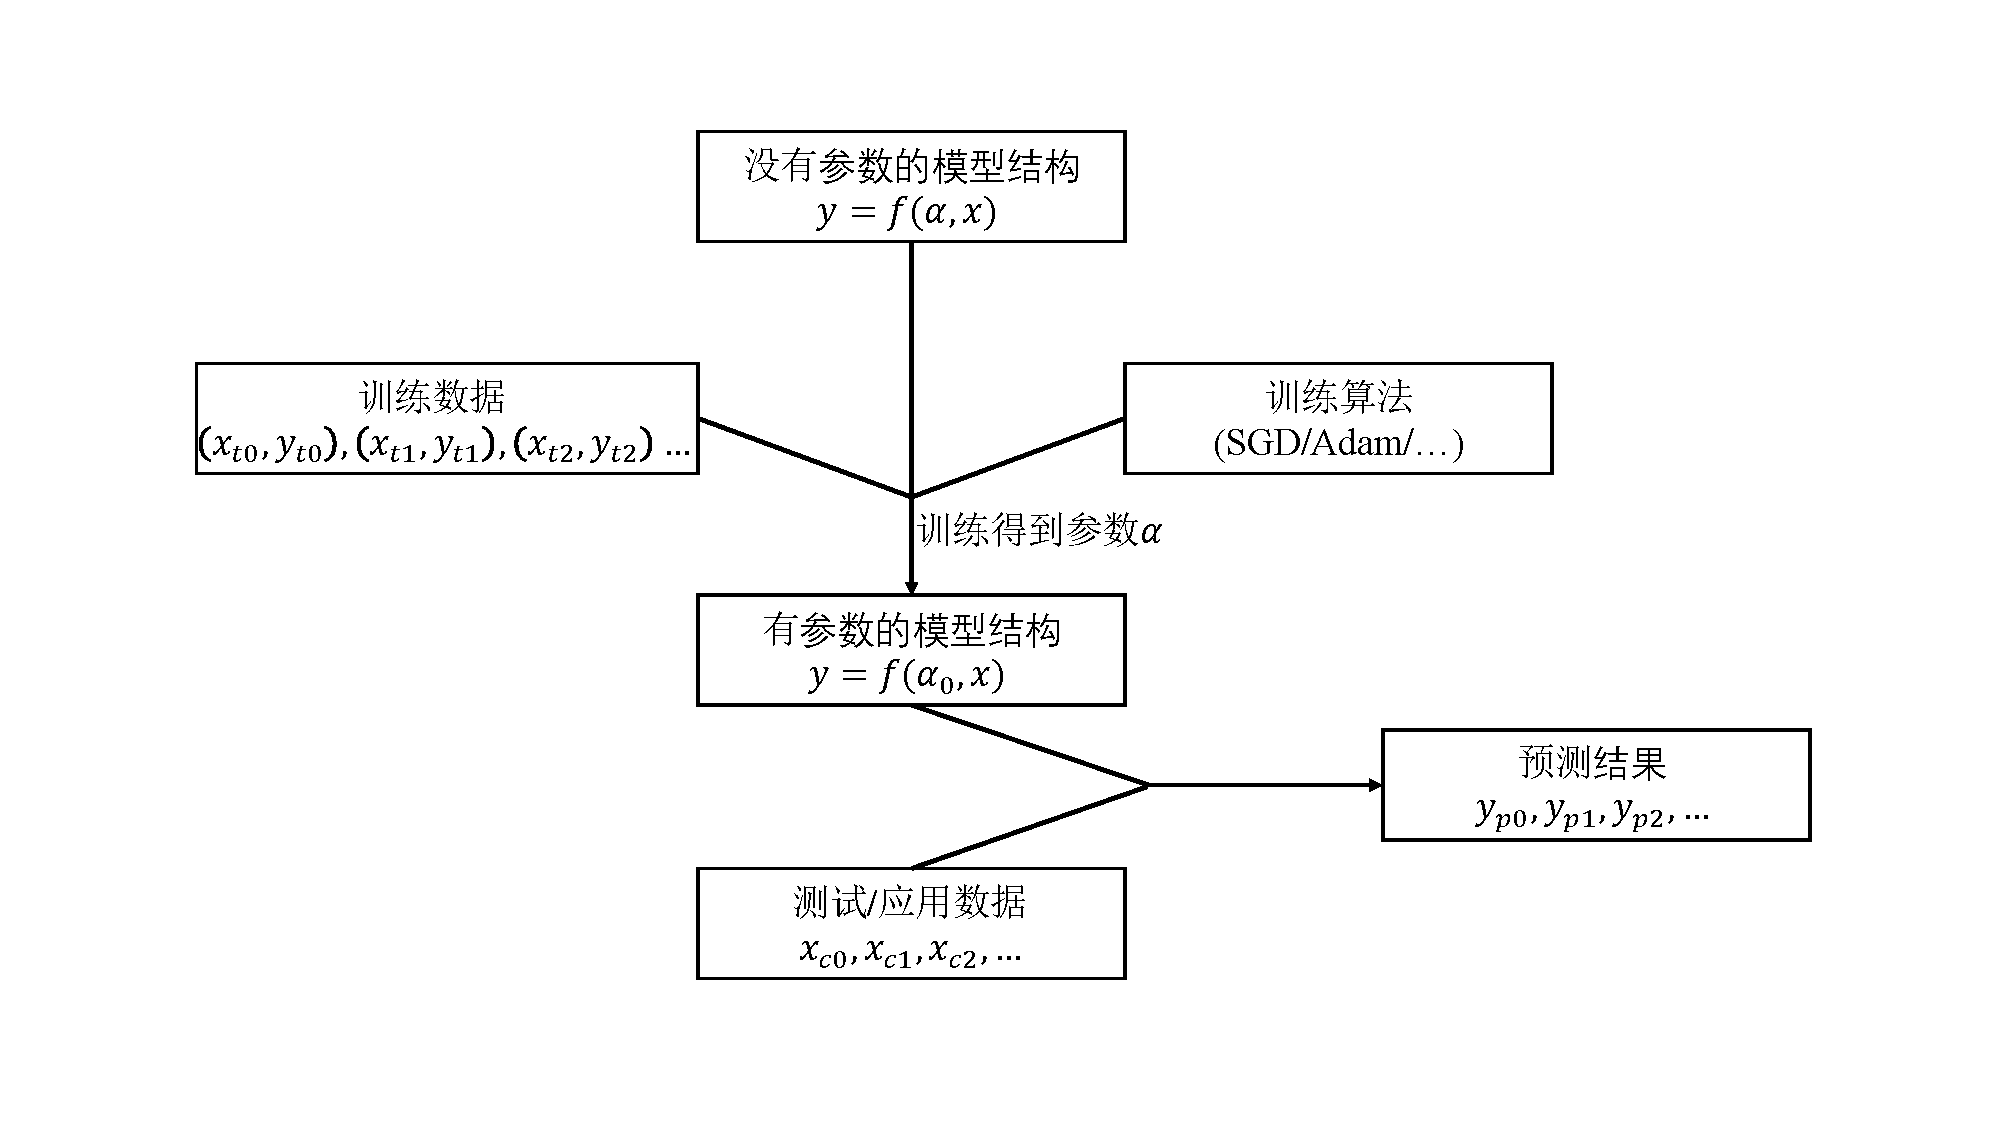
\includegraphics[width = 1.\textwidth]{chap/img/model_learning.pdf}
    \caption{使用训练数据,将没有参数的模型$f(\alpha,x)$训练至有参数,可以实际应用的模型$f(\alpha_0,x)$的过程}
    \label{fig:model_learning}
\end{figure}
几乎所有的深度神经网络都需要配合训练(training)得到的参数才能应用,即预测.不同的训练会得到不同的参数,预测得到的结果也会不同.
\par
梯度下降法是最典型的模型训练方法.
\par
反向传播是常用的深度神经网络求梯度的方法.

\section{视频跟踪算法}
上一章中介绍过,视频跟踪算法接受图像序列,输出目标位置.具体的,对于一个$n$帧长的,由$pic_1,pic_2...pic_n$共$n$张图像组成的视频,使用跟踪算法$Track$进行跟踪,在第$t$时刻算法的计算可以用下面的公式表示:
\par
\begin{equation}\label{equ:track_ite}  P_t,S_t=Track(pic_{t},P_{t-1},S_{t-1})  \end{equation}
\par
其中$P_t$,$S_t$分别代表$t$时刻的\textbf{目标位置与形态}和\textbf{跟踪状态}.这两个概念将在本节后边介绍.
\par
在整个跟踪过程中,跟踪系统将在每一帧到来时执行公式\ref{equ:track_ite}中描述的过程,最终获得所有的目标位置与形态$P$.
\par
\subsection{目标位置与形态的描述} 
所有目标跟踪算法都有明确的\textbf{目标位置与形态的描述}方法.事实上,这种描述基本可以等同于目标跟踪算法的输出形式.典型的目标位置与形态描述有矩形式和像素级的.
\par
\subsubsection{矩形式目标位置与形态描述}
\par
\begin{figure}[htbp!]
    \centering
    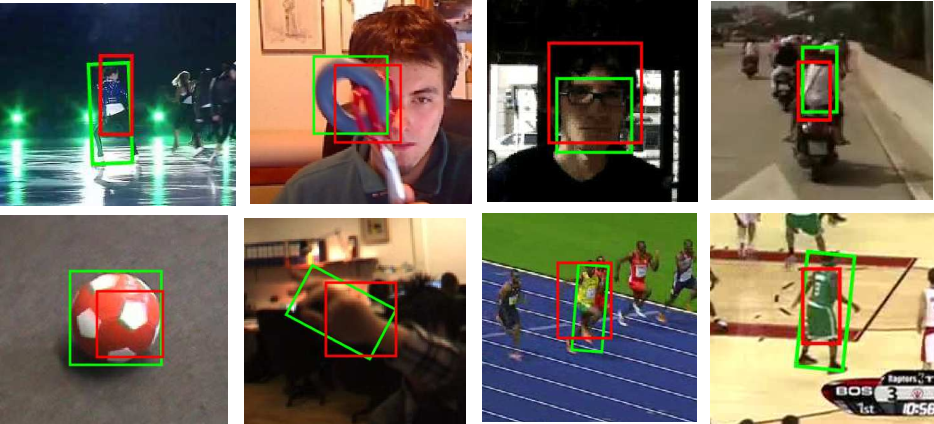
\includegraphics[width = 1.\textwidth]{chap/img/overlap_examples.pdf}
    \caption{图片为VOT竞赛中描述标记与目标的插图\supercite{VOT_TPAMI},这里用于演示矩形式目标描述中描述目标的外包矩形.红色:限定竖直的的外包矩形;绿色:不限定竖直的外包矩形.}
    \label{fig:bunding_boxes}
\end{figure}
\par
常见的矩形框视频目标跟踪算法考虑会考虑目标的最小外包矩形(Bounding Box)和位置(Location).最小外包矩形的方向有时是限定为竖直的,即矩形的上下边平行于图像的上下边,左右边同理;有时不限定,可以是任何方向.限定竖直与不限定竖直的矩形表示法如图\ref{fig:bunding_boxes}所示.位置一般用矩形的中心表示.
\par
\subsubsection{像素级目标位置与形态描述}
像素级跟踪算法的运动模型需要表达的信息与矩形框跟踪算法类似,但信息更为细节.像素级目标描述没有矩形式目标描述那样用矩形的中心描述目标的位置,用矩形的形状描述目标的形状.而是直接用二值的,覆盖全图的像素来同时描述目标的位置与形状.
% TODO 此处应有图演示像素级描述方式

\subsection{跟踪状态}
\textbf{跟踪状态}是跟踪模型在跟踪过程中,用于记录当前信息以继续跟踪的状态量.在$t$时刻的跟踪状态$S_t$,它的物理含义可能包含用于预估目标将来的运动的目标之前一段时间的运动与变化状态.通常情况下,跟踪模型预测新一帧的目标位置需要用该帧到来时刻的跟踪状态与该帧的图像,但如果跟踪状态描述得足够理想,很多情况下仅凭描述优秀的跟踪状态就可猜测出目标接下来的运动趋势,从而大致确定新的目标位置与形态.
\par
多数基于深度学习的视频目标跟踪算法都使用RNN的状态量存储目标跟踪状态.
\par

% TODO 介绍经典跟踪算法